\documentclass[a4paper, 12pt]{article}

\usepackage[left=2cm,right=2cm,
top=2cm,bottom=2cm,bindingoffset=0cm]{geometry}

\usepackage[T2A]{fontenc}
\usepackage[utf8]{inputenc}
\usepackage{color}
\usepackage{graphicx}
\usepackage{caption}
\usepackage{listings}
\usepackage{subcaption}
\usepackage{tikz}
\usepackage{float}
\usepackage[english, russian]{babel}
\usepackage{amsmath,amsfonts,amssymb,amsthm,mathtools}
\usepackage{lscape}

\begin{document}
	\begin{center}
		\textbf{\textit{Задание}}
	\end{center}
	
	\begin{enumerate}
		\item Построить функции формы с помощью аппроксимации Лагранжа и Серендипова семейства для квадратичного четырехугольного элемента 
		\item Вычислить производные от функций форм $\dfrac{\partial N_i}{\partial x}, \dfrac{\partial N_i}{\partial y}$
		\item Вычислить интеграл $\displaystyle \iint\limits_S \left(\dfrac{\partial N_i}{\partial x}\cdot \dfrac{\partial N_i}{\partial y}\right)\, dS$
	\end{enumerate}
	\begin{figure}[H]
		\centering
		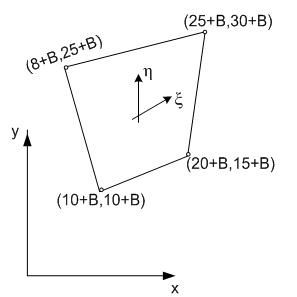
\includegraphics[width=0.3\linewidth]{task.png}
	\end{figure}

	\begin{center}
		\textbf{\textit{Решение}}
		
		\textbf{В = 7}
	\end{center}
	\begin{figure}[H]
		\centering
		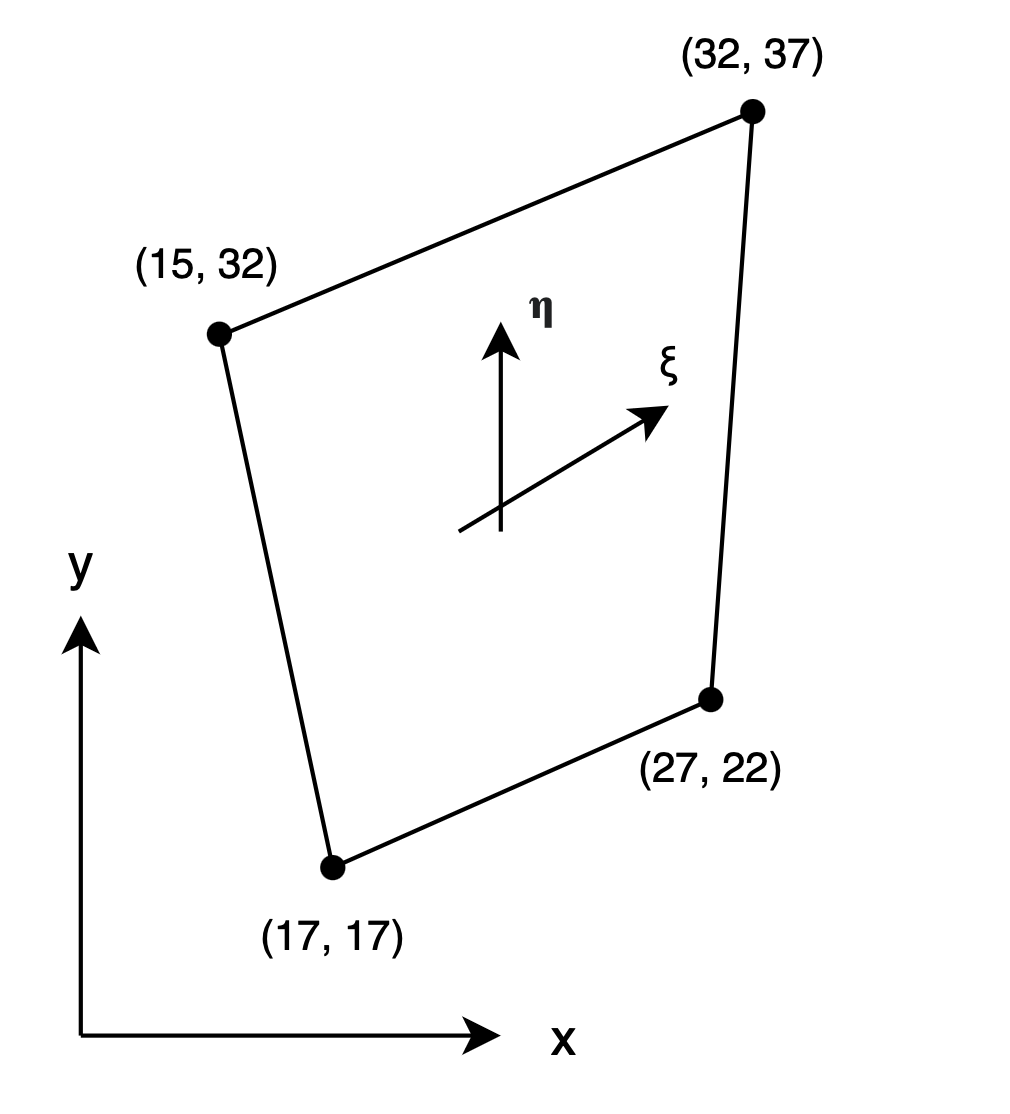
\includegraphics[width=0.3\linewidth]{mytask.png}
	\end{figure}
	
	В естественной системе координат:
	\begin{figure}[H]
		\centering
		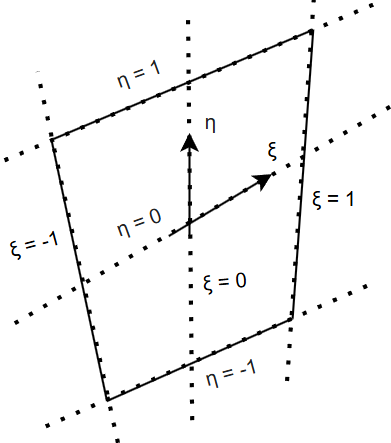
\includegraphics[width=0.3\linewidth]{ncs.png}
	\end{figure}
	\begin{center}
		\begin{tikzpicture}
			\draw(0,0) -- (4,0) -- (4,3) -- (0,3) -- cycle;
			\draw[->] (0,1.5) -- (5, 1.5) node[below right] {$\xi$};
			\draw[->] (2,0) -- (2,4) node[right] {$\eta$};
			\fill (0,0) circle(1.5pt);
			\fill (2,0) circle(1.5pt);
			\fill (4,0) circle(1.5pt);
			\fill (4,1.5) circle(1.5pt);
			\fill (0,1.5) circle(1.5pt);
			\fill (4,3) circle(1.5pt);
			\fill (2,3) circle(1.5pt);
			\fill (0,3) circle(1.5pt);
			\fill (2,1.5) circle(1.5pt);
			\node at (0,-0.5) {\footnotesize 1};
			\node at (2,-0.5) {\footnotesize 2};
			\node at (4,-0.5) {\footnotesize 3};
			\node at (4.25,1.75) {\footnotesize 4};
			\node at (4.25,3.25) {\footnotesize 5};
			\node at (1.75,3.25) {\footnotesize 6};
			\node at (-0.25,3.25) {\footnotesize 7};
			\node at (-0.25,1.75) {\footnotesize 8};
			\node at (2.25,1.75) {\footnotesize 0};
		\end{tikzpicture}
	\end{center}

	\begin{center}
		\textbf{\textit{Лагранжево семейство}}
	\end{center}

	\begin{center}
		\begin{tikzpicture}
			\draw(0,0) -- (4,0) -- (4,3) -- (0,3) -- cycle;
			\fill (0,0) circle(1.5pt);
			\fill (2,0) circle(1.5pt);
			\fill (4,0) circle(1.5pt);
			\fill (4,1.5) circle(1.5pt);
			\fill (0,1.5) circle(1.5pt);
			\fill (4,3) circle(1.5pt);
			\fill (2,3) circle(1.5pt);
			\fill (0,3) circle(1.5pt);
			\fill (2,1.5) circle(1.5pt);
			\node at (0,-0.5) {\footnotesize $\xi_i=-1$};
			\node at (2,-0.5) {\footnotesize $\xi_1=0$};
			\node at (4,-0.5) {\footnotesize $\xi_2=1$};
	
			\node at (-0.75,3.25) {\footnotesize $\eta_2=1$};
			\node at (-0.75,1.75) {\footnotesize $\eta_1=0$};
			\node at (-0.75,0.25) {\footnotesize $\eta_i=-1$};
	
			\draw(0.5,0.5) circle(8pt);
			\node at (0.5,0.5) {\footnotesize 1,1};
	
			\draw(0.5,1.75) circle(8pt);
			\node at (0.5,1.75) {\footnotesize 1,2};
		\end{tikzpicture}
	\end{center}

	Функция формы:
	\[
	N_{ij}=L_i^n(\xi)L_j^m(\eta)
	\]

	$L_i^n(\xi)L_j^m(\eta)$ - многочлены Лагранжа, $n,m$ - количество разбиений по $\xi, \eta$

	\[
		L_i^n(\xi)=\frac{(\xi-\xi_1)(\xi-\xi_2)\dots(\xi-\xi_n)}{(\xi_i-\xi_1)(\xi_i-\xi_2)\dots(\xi_i-\xi_n)}
	\]
	\[
		N_{ij}=L_i^2(\xi)L_j^2(\eta),\ i \neq 1,2
	\]
	\[
		L_i^2(\xi)=\frac{(\xi-\xi_1)(\xi-\xi_2)}{(\xi_i-\xi_1)(\xi_i-\xi_2)}
	\]
	\[
		N_{11}=\frac{\xi\cdot(\xi-1)}{-1\cdot(-2)}\cdot \frac{\eta\cdot(\eta-1)}{-1\cdot(-2)}=\frac{1}{4}\cdot\xi\cdot\eta (\xi-1)(\eta-1)
	\]
	\[
		N_{12}=\frac{\xi\cdot(\xi-1)}{2}\cdot \frac{(\eta+1)(\eta-1)}{1\cdot(-1)} = -\frac{1}{2} \xi(\xi - 1)(\eta^2 - 1)
	\]

	\begin{center}
		\textbf{\textit{Серендипово семейство}}
	\end{center}
	\[
		\varphi_2=\alpha_1+\alpha_2x+\alpha_3y+\alpha_4xy+\alpha_5x^2y+\alpha_6xy^2+\alpha_7x^2+\alpha_8y^2 
	\]
	
\end{document}